\section{Problem}\label{sec:problem}

In our setting we assume users own an Internet enabled mobile device with positioning capabilities. Users issue \spath queries to an online service provider. Users want the response time, on the return of their \spath result, to be comparable to that of an offline application. We use the terms user query, incoming query, and query interchangeably.

The \spath service provider needs to provide a fast service to its users. The service provider also want to save cost on hardware, such as CPU and HDD space. The \spath provider therefor wants to return as many \spath results as possible, using the least amount of computation and space.

Calculating a \spath will, regardless of the algorithm used, always be an expensive calculation\cite{CNeed}. Using a \spath cache at the \spath service provider can reduce the CPU cycles used in order to return a \spath result. Doing so would at the same time also increase the response time of the \spath service, as saving CPU cycles not only allows for more \spaths to be computed on the same hardware, but also allows for returning a cached result much faster than it would be possible if the \spath had to be calculated first.

A \spath has the property of \oss (see lemma \ref{lem:oss}) which means that any \spath in the cache can answer any \spath query where both origin and target node are on the \spathns. Calculating which \spathsns, and their sub-paths, provide the most benefit will obviously be necessary for optimal utilization of the cache. A static cache, which is populated in an offline phase (fig. \ref{fig:routequery}E), is used. A static cache will impose minimal overhead to query processing. Section \ref{sec:competitors} explains why we choose a static cache.

The properties of \ossns (Lemma \ref{lem:oss}) states that all sub-paths on a \spath are also \spathsns. Using \spath Q1 in table \ref{tab:queries} we would also be able to a query from $v_3$ to $v_5$, or $v_4$ to $v_6$ (See fig. \ref{fig:rxmap}), as these nodes are part of Q1. The same of cause also holds for any \spath Q1-Q6 from table \ref{tab:queries}.

\begin{figure}[hbt]
  \center
        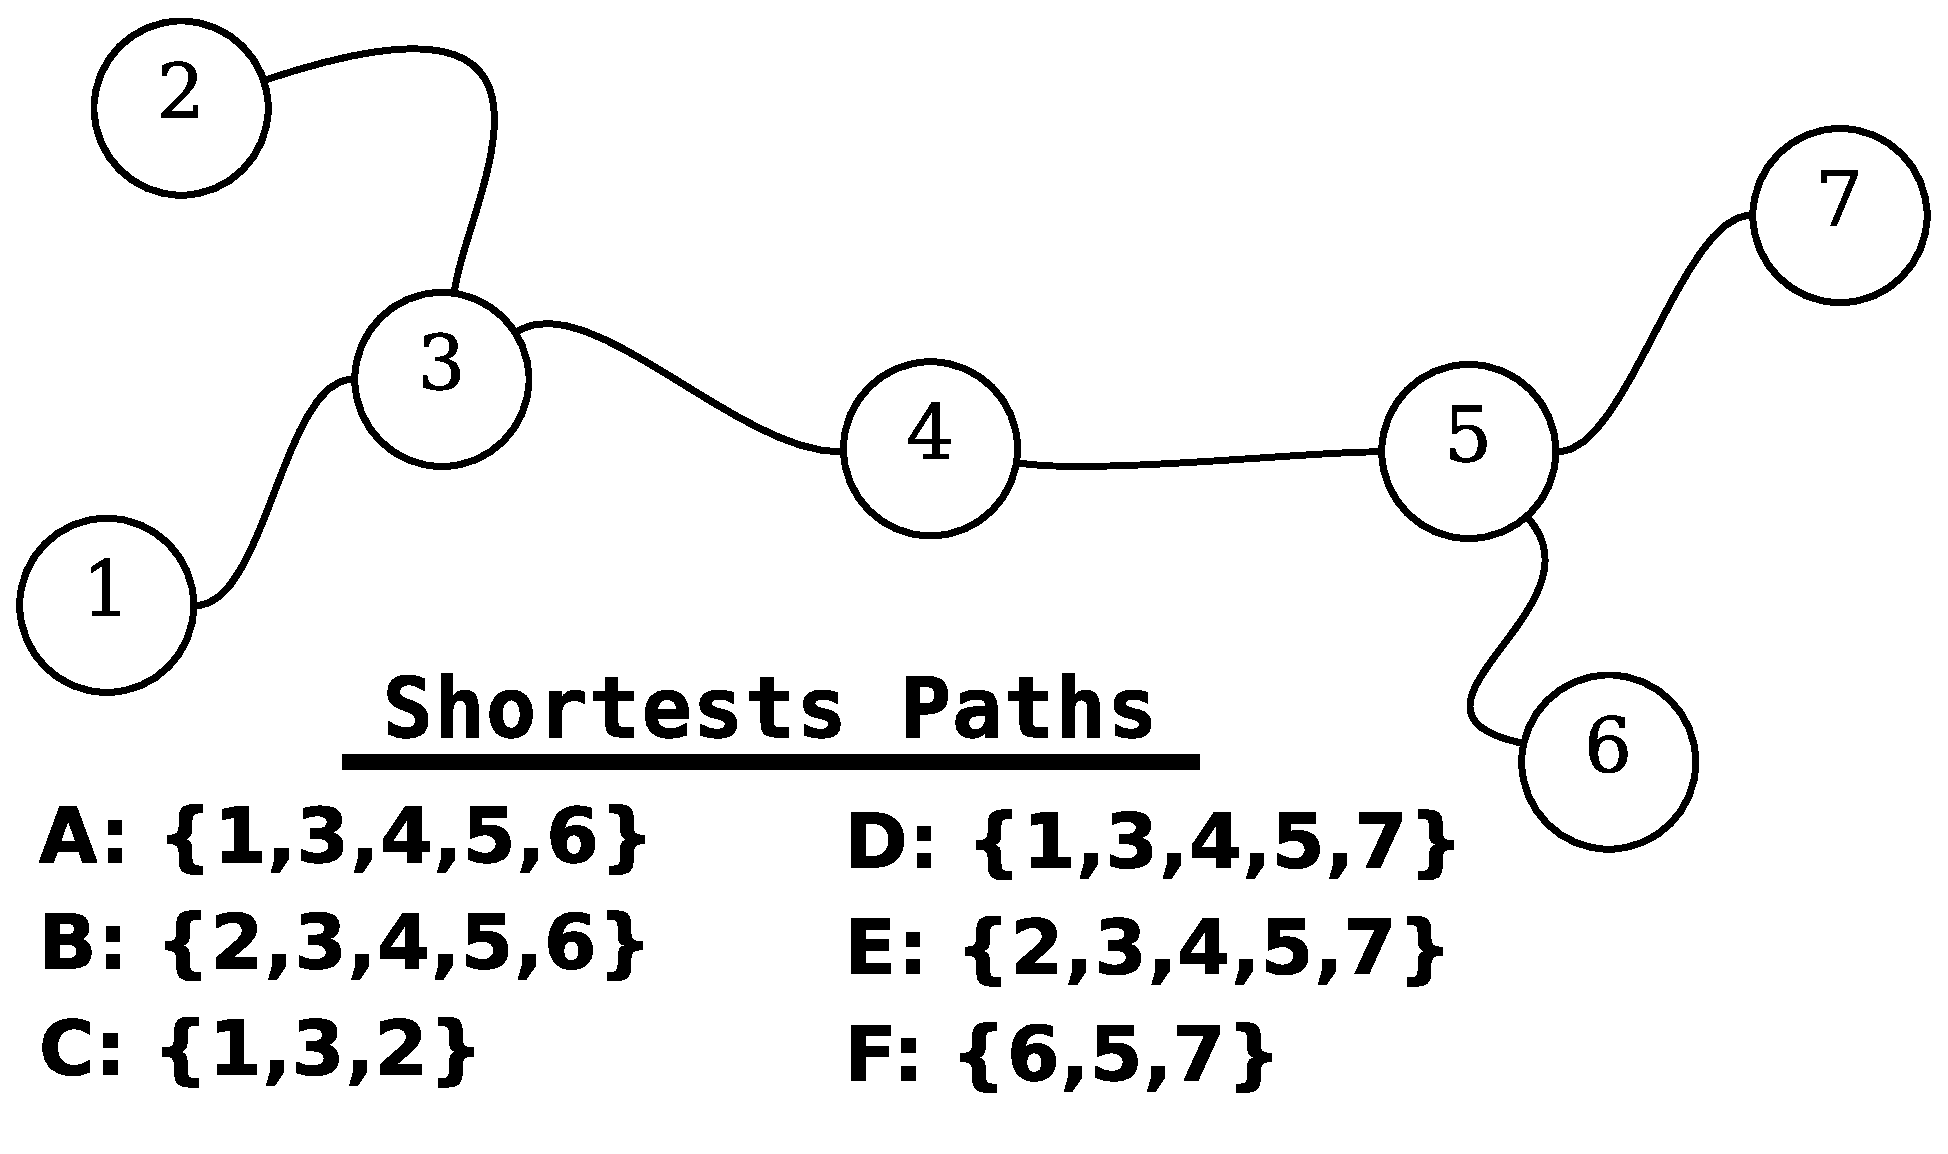
\includegraphics[width=0.5\textwidth]{figures/rxmap}
        \caption{Simple graph representation of a map.}
  \label{fig:rxmap}
\end{figure}


\subsection{Architecture}
We propose a system with a static \spath cache implemented in front of an existing \spath service (See fig. \ref{fig:routequery}) such that if the cache can answer a query then the result can be returned immediately. 

When the system receives a \spath query from a user (fig. \ref{fig:routequery}A) the system first checks if the cache (fig. \ref{fig:routequery}B) is able to answer the query. If the cache contains the query answer it is immediately returned (fig. \ref{fig:routequery}D), else the \spath algorithm is called (fig. \ref{fig:routequery}C) and the \spath result returned (fig. \ref{fig:routequery}D).

\begin{figure}
  \center
        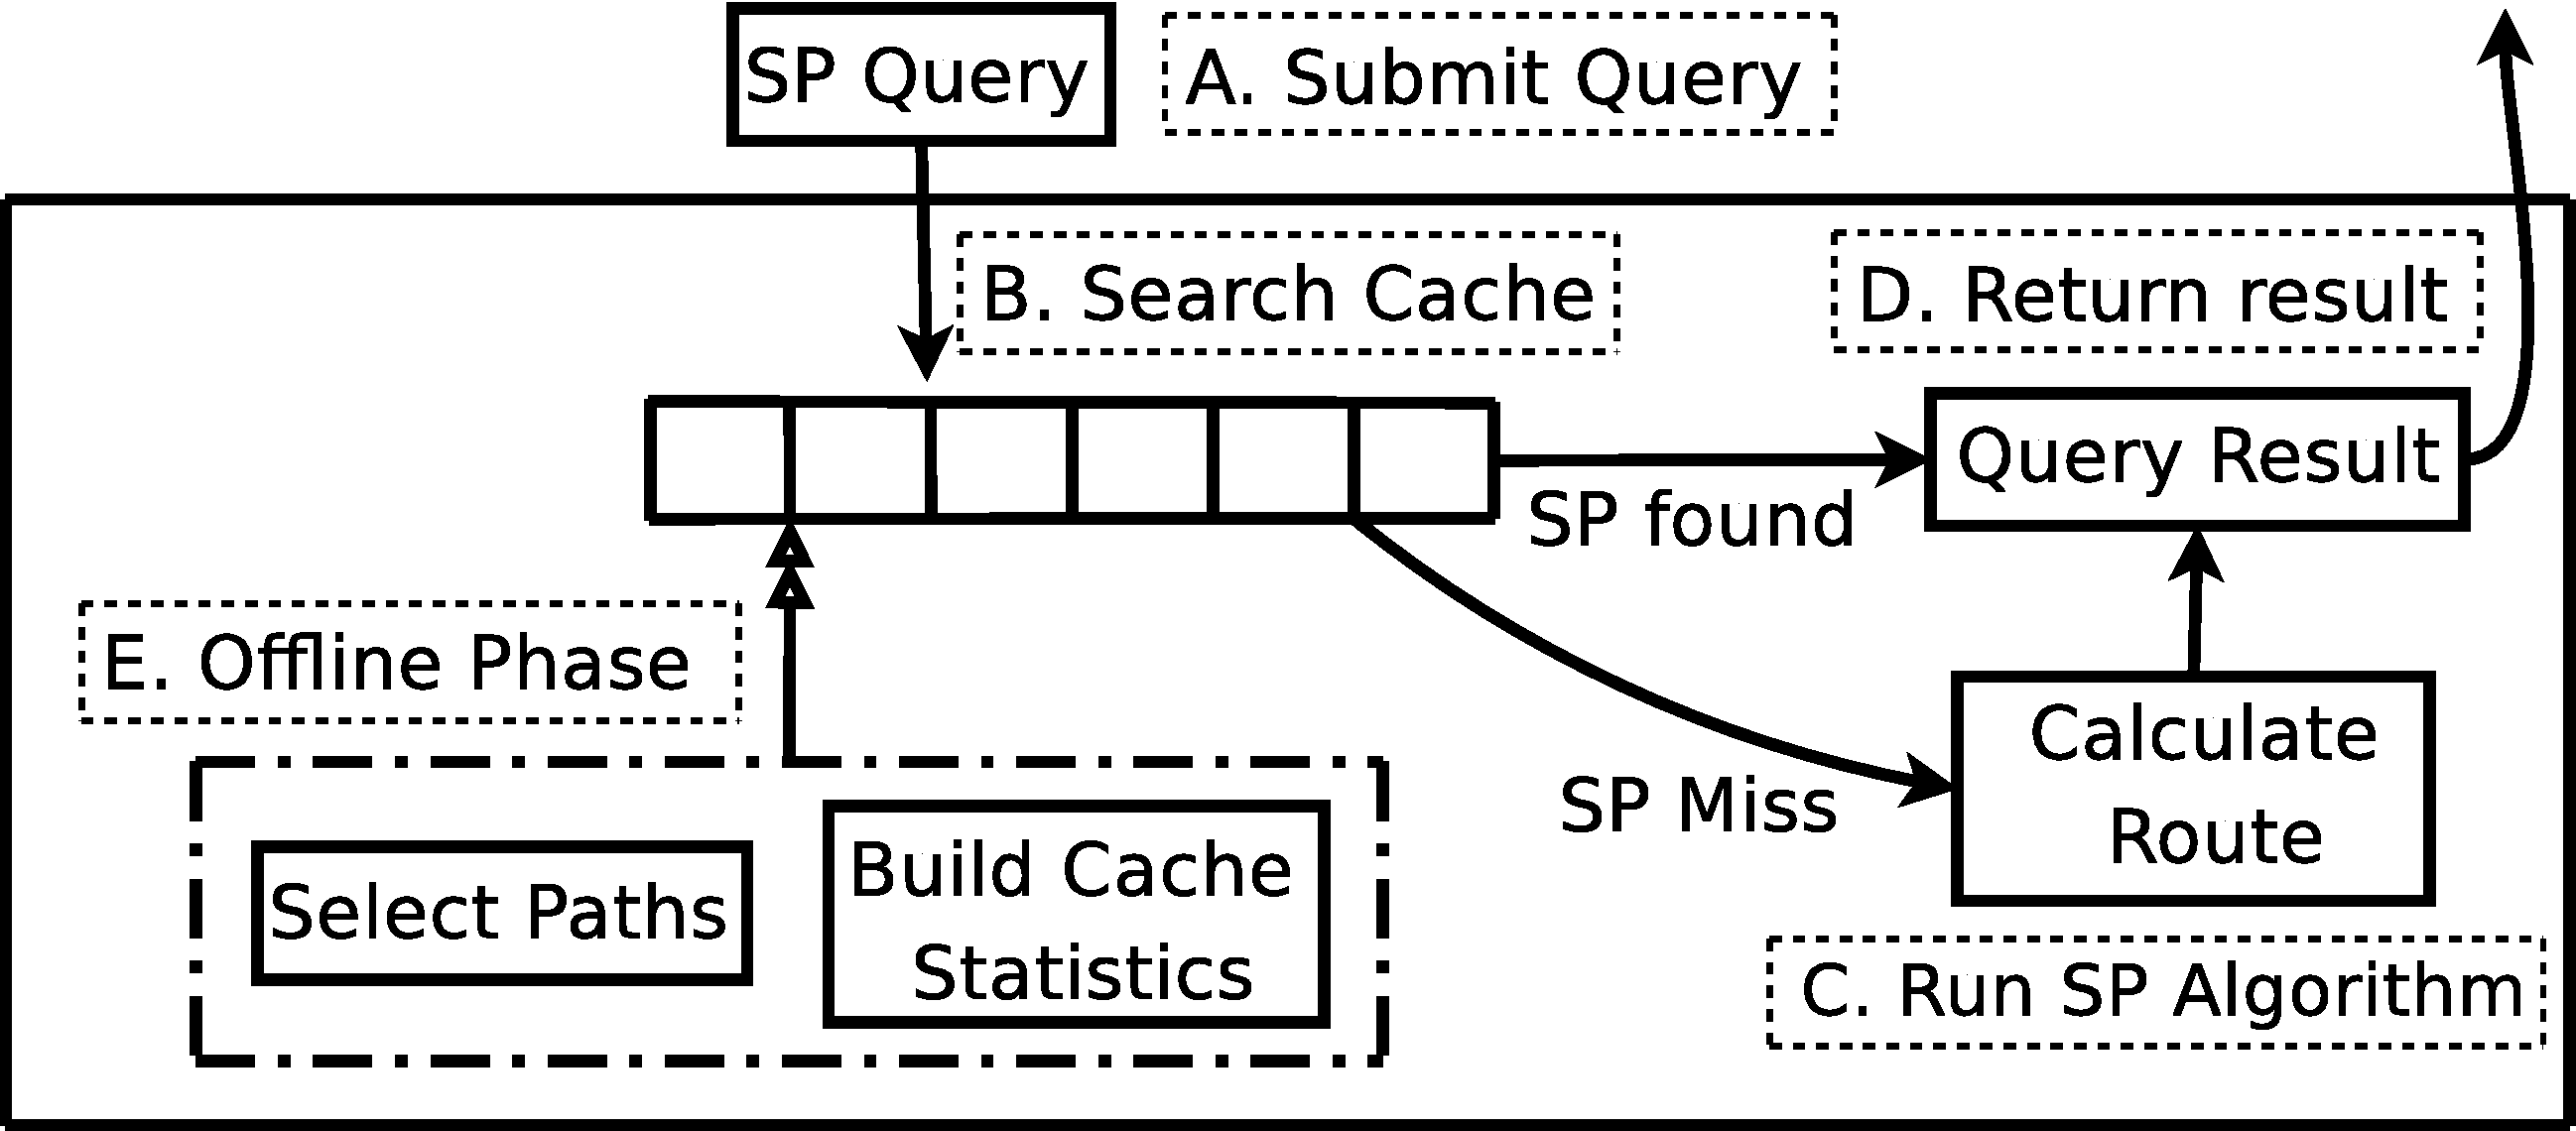
\includegraphics[width=0.5\textwidth]{figures/routequery}
        \caption{Buffer placement in \spath service providers system.}
  \label{fig:routequery}
\end{figure}


\subsection{Optimization Intend} \label{subsec:goals}

As the main problem with expensive \spath calculations is time needed, we use reduction in \textit{\cet} as the main optimization target and measurement to evaluate our success.
At a \spath service provider, the time spent to return a \spath result is essentially composed of two tasks: calculating the \spath and the overhead of query processing. 

We will address 3 subgoals:
\begin{enumerate}
\item \label{item:goal1}Reduce the gross \cet used to calculate \spathsns.
\item \label{item:goal2}Reduce the gross \cet spent on overhead in query processing.
\item \label{item:goal3}Determine the value of a sub-path in the cache.
\end{enumerate}

We want reduce the gross \cet of \spath calculations - goal 1 - as it is the most CPU intensive task at a \spath service, and therefor also the most time consuming. By using a cache we expect to see a negavite correlation between cache hit rate and \cet used on \spath calculation.

In a \spath service there will always be a some overhead associated with \spath query processing. Introducing a cache in front of the existing \spath service (fig. \ref{fig:routequery}B) will undeniably add more overhead as the cache needs to be queried for all queries submitted to the \spath service, regardless of whether it is able to answer the query or not. In order for the cache to be useful, the overhead introduced needs to be minimized (goal \ref{item:goal2}). We always have to make sure that the savings achieved by adding a cache to the system is greater than the overhead introduced.

The fact that the system will be using a static cache, and \spaths exhibit the \oss property, makes goal 3 - determining the value of a \spath subpath - very important. The ability to do goal \ref{item:goal3} well will have a direct influence on goal \ref{item:goal1} and  \ref{item:goal2}. If we fill the cache with useless \spaths we will end up calculating a \spath for all queries, as well as the overhead from checking the cache for each query. Solving goal 3 well is the most direct way to solve goal 1.

The \oss property states that every sub-path of a \spath is also a \spath. i.e \spath Q1 in table \ref{tab:queries} consists of: 
$\{SP_{1,3}, SP_{1,4}, SP_{1,5}, SP_{1,6}, SP_{3,4},$ $SP_{3,5}, SP_{3,6}, SP_{4,5}, SP_{4,6}, SP_{5,6}\}$, each one being a \spathns.

\begin{lemma}\label{lem:oss}
If a path $SP_{s,t}: v_s,v_{s+1},\ldots,v_t$ is a \spath, then $\forall$ $(v_k,v_l) | v_k \in SP_{s,t} \wedge v_l \in SP_{s,t}$ there is a  \spath $SP_{k,l}$ with start-/end-node in $v_k,v_l$, following a sub-path of $SP_{s,t}$ 
\end{lemma}

\begin{table}
\begin{tabular*}{\columnwidth}{|l||p{0.69\columnwidth}|}
\hline
\bf Abbreviation & \bf Meaning \\\hline
\spath          & Shortest Path \\\hline
$SP_{s,t}$	& \spathns: $\{v_s,v_{s+1},\ldots,v_t\}$ \\\hline
\acs{LRU}       & \acl{LRU} \\\hline
FIFO            & First In First Out \\\hline
\acs{SPS}       & \acl{SPS} \\\hline
\acs{CET}	& \acl{CET} \\\hline
\acs{OSS}	& \acl{OSS} \\\hline
\end{tabular*}
\caption{Table of Notation}
\label{tab:symbols}
\end{table}




% \subsection{helping text}
% \begin{enumerate}
% \item Introduce the problem setting in more detail than in the introduction and formally define the problem and what exactly we aim to solve in this paper.\\
% \item show where exactly the proposed cache is located in an online \spath service providers system.
% \item State goal 1(a) and 2(b)
% 	\begin{enumerate}
% 	\item Reduce the time spent executing the \spath algorithm. - The \spath algorithm is usually the single most CPU expensive task at a \spath service provider.
% 	\item Reduce the time spent on overhead. - Introducing a cache will also add some overhead, this overhead not desirable and should  be minimized.
% 	\end{enumerate}
% \item Introduce the overall setting which our solution work in and give a table of notation for reader reference.
% \end{enumerate}
